\documentclass{article}\usepackage[]{graphicx}\usepackage[]{xcolor}
% maxwidth is the original width if it is less than linewidth
% otherwise use linewidth (to make sure the graphics do not exceed the margin)
\makeatletter
\def\maxwidth{ %
  \ifdim\Gin@nat@width>\linewidth
    \linewidth
  \else
    \Gin@nat@width
  \fi
}
\makeatother

\definecolor{fgcolor}{rgb}{0.345, 0.345, 0.345}
\newcommand{\hlnum}[1]{\textcolor[rgb]{0.686,0.059,0.569}{#1}}%
\newcommand{\hlstr}[1]{\textcolor[rgb]{0.192,0.494,0.8}{#1}}%
\newcommand{\hlcom}[1]{\textcolor[rgb]{0.678,0.584,0.686}{\textit{#1}}}%
\newcommand{\hlopt}[1]{\textcolor[rgb]{0,0,0}{#1}}%
\newcommand{\hlstd}[1]{\textcolor[rgb]{0.345,0.345,0.345}{#1}}%
\newcommand{\hlkwa}[1]{\textcolor[rgb]{0.161,0.373,0.58}{\textbf{#1}}}%
\newcommand{\hlkwb}[1]{\textcolor[rgb]{0.69,0.353,0.396}{#1}}%
\newcommand{\hlkwc}[1]{\textcolor[rgb]{0.333,0.667,0.333}{#1}}%
\newcommand{\hlkwd}[1]{\textcolor[rgb]{0.737,0.353,0.396}{\textbf{#1}}}%
\let\hlipl\hlkwb

\usepackage{framed}
\makeatletter
\newenvironment{kframe}{%
 \def\at@end@of@kframe{}%
 \ifinner\ifhmode%
  \def\at@end@of@kframe{\end{minipage}}%
  \begin{minipage}{\columnwidth}%
 \fi\fi%
 \def\FrameCommand##1{\hskip\@totalleftmargin \hskip-\fboxsep
 \colorbox{shadecolor}{##1}\hskip-\fboxsep
     % There is no \\@totalrightmargin, so:
     \hskip-\linewidth \hskip-\@totalleftmargin \hskip\columnwidth}%
 \MakeFramed {\advance\hsize-\width
   \@totalleftmargin\z@ \linewidth\hsize
   \@setminipage}}%
 {\par\unskip\endMakeFramed%
 \at@end@of@kframe}
\makeatother

\definecolor{shadecolor}{rgb}{.97, .97, .97}
\definecolor{messagecolor}{rgb}{0, 0, 0}
\definecolor{warningcolor}{rgb}{1, 0, 1}
\definecolor{errorcolor}{rgb}{1, 0, 0}
\newenvironment{knitrout}{}{} % an empty environment to be redefined in TeX

\usepackage{alltt}
\usepackage[brazil]{babel}
\usepackage{kpfonts}
\usepackage{indentfirst}
\usepackage{parskip}
\usepackage{graphicx}
\usepackage{float}
\graphicspath{ {img/} }
\usepackage{amsmath}
\usepackage{array}
\usepackage{booktabs,caption}
\usepackage[autostyle]{csquotes}
\usepackage{siunitx}

\sisetup{
round-mode = places,
round-precision = 2,
output-decimal-marker={.},
group-separator ={,},
group-minimum-digits = 3
}

\newenvironment{conditions}
  {\par\vspace{\abovedisplayskip}\noindent\begin{tabular}{>{$}l<{$} @{${}={}$} l}}
  {\end{tabular}\par\vspace{\belowdisplayskip}}


\usepackage{multirow}


\title{Sistema Financeiro Nacional}
\author{FIA Business School}
\IfFileExists{upquote.sty}{\usepackage{upquote}}{}
\begin{document}
\maketitle

\section*{Sistema Financeiro Nacional}

Pense no Sistema Financeiro Nacional (SFN) como um \enquote{motor de automóvel} com três grandes partes:

\begin{itemize}

  \item \textbf{Bloco do motor}. \enquote{Define} o tamanho do motor; podemos associá-lo aos \textit{órgãos governamentais} (conselhos);

  \item \textbf{Cabeçote}. \enquote{Controla e limita}  a atuação dos pistões; podemos associá-lo às \textit{autarquias governamentais} e

  \item \textbf{Pistões}. \enquote{Partes móveis}, pois têm seu movimento originado pela explosão da gasolina; 
        podemos associá-los às \textit{Instituições Financeiras}.

\end{itemize}

Em nosso exemplo, quem coloca a gasolina e acelera para promover o movimento dos pistões (IFs) são as pessoas 
(físicas e jurídicas). O movimento gerado aos pistões pode ser tanto para frente quanto para trás. 
Vamos associar o interesse pelo movimento aos poupadores e tomadores.\par

\textbf{Importante}. As IFs podem ser empresas privadas (como os grandes Bancos Múltiplos Nacionais e Estrangeiros) 
ou públicas (como o BNDES ou a Caixa Econômica Federal) ou estatais (economia mista, como o Banco do Brasil) e sua 
importância está na capacidade de intermediação financeira entre poupadores e tomadores.\par

A intermediação financeira é a capacidade que as IFs têm de:

\textbf{captar recursos dos poupadores e emprestá-los aos tomadores}: neste caso as IFs ganham juros 
(spread bancário) pelo risco que correm na intermediação financeira. Tais operações fazem parte do 
\enquote{Mercado de Crédito} (Figura 1). Também é correto dizermos que o mercado de crédito é de curto prazo.

\begin{figure}[H]
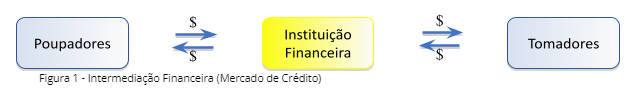
\includegraphics[width=12cm]{mercado-de-credito}
\centering
\label{mercado-de-credito}
\caption{Mercado de crédito.}
\end{figure}
  
\textbf{vender títulos e valores mobiliários emitidos por tomadores diretamente aos poupadores}: neste caso, 
as IFs cobram comissões pela intermediação financeira;  tais operações fazem parte do \enquote{Mercado de Capitais} 
(Figura 2). Também é correto dizermos que o mercado de capitais é de longo prazo.

\begin{figure}[H]
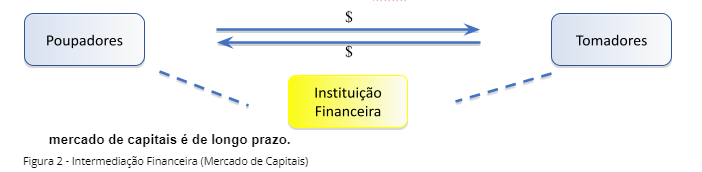
\includegraphics[width=12cm]{mercado-de-capitais}
\centering
\label{mercado-de-capitais}
\caption{Mercado de capitais.}
\end{figure}

Podemos concluir que a \textbf{Intermediação Financeira} é o importante trabalho das IFs em atender:

\begin{itemize}

  \item quem tem dinheiro disponível para aplicar e quem precisa tomar dinheiro emprestado  e

  \item quem quer vender um ativo financeiro e quem quer comprá-lo.

\end{itemize}

O \textbf{SFN} tem como objetivo contínuo promover e garantir as atividades que envolvam intermediação financeira,
pois sem ela os poupadores não teriam segurança para aplicar suas sobras de recursos e os tomadores teriam
dificuldade em encontrar quem os financiasse. Também haveria dificuldade em negociar (compra e venda) de
títulos e valores mobiliários, algo que seria muito grave para o financiamento da produção do país.\par

Para promover e garantir a intermediação financeira, o SFN é composto dos chamados:

\begin{itemize}
  \item \textbf{Subsistema Normativo}: conselhos formados por pessoas (investidas em cargos públicos ou não)
        que normatizam e autarquias (espécies de empresas públicas) que controlam e fiscalizam;

  \item \textbf{Subsistema Operativo}: instituições (é o próprio mercado em si) que executam diversas
        operações financeiras, como:

        \begin{itemize}

          \item circulação de moeda (em geral pagamentos e recebimentos);

          \item concessão de crédito (em geral empréstimos e financiamentos);

          \item captação de recursos (em geral investimentos);

          \item emissão, negociação e custódia de títulos e valores mobiliários (mercado de capitais);

          \item proteção de riscos (em geral hedge);

          \item câmbio (em geral troca de moedas);

          \item estruturação de operações de compra e venda de empresas (em geral quando envolve grandes empresas/negócios);

          \item seguros privados (em geral de bens e vida);

          \item previdência complementar, que pode ser fechada e aberta a qualquer pessoa (em geral para aposentadoria)  e

          \item serviços financeiros (em geral prestação de serviços que diversas instituições fazem, por exemplo,
                coleta e custódia de valores).

        \end{itemize}

\end{itemize}

A Figura 3 representa o relacionamento entre os subsistemas e as responsabilidades genéricas dos respectivos entes.

\begin{figure}[H]
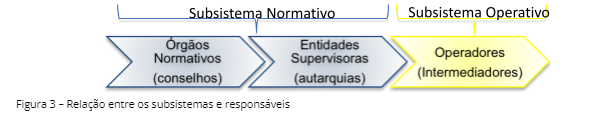
\includegraphics[width=12cm]{sfn-subsistemas}
\centering
\label{sfn-subsistemas}
\caption{Relação entre os subsistemas do SFN.}
\end{figure}

\section*{Operadores}

Os Operadores (Subsistema Operativo) são formados por instituições de natureza privada (S.A.s e Ltd..as), 
públicas (na empresa pública, o único acionista é o governo) ou estatais (S.A.s de economia mista com 
capital público e privado). Independente de sua natureza, todas elas realizam algum tipo de intermediações 
financeiras que vão desde os mais simples e clássicos, como captação de investimentos (de poupadores) e 
empréstimos (para tomadores), até os mais complexos, como estruturação e venda de TVM de empresas 
(tomadoras) para investidores (poupadores).\par

Os Operadores estão divididos de acordo com as atividades que realizam. Na Tabela 1 temos a lista completa.

\begin{table}[H]
\centering
\caption{Diferentes tipos de Operadores.}
\resizebox{\textwidth}{!}{%
\begin{tabular}{ |p{2cm}|p{2cm}|  }
 \hline
 \multicolumn{2}{|c|}{Subsistema Operativo}\\
 \hline
 \textbf{Espécie}                                                               & \textbf{Operadores (atividades)}\\
 \hline
 \multicolumn{1}{|l|}{Instituição Financeira Captadora de Depósito à Vista}     & \multicolumn{1}{l|}{Bancos Comerciais}\\
 \hline
 \multicolumn{1}{|l|}{Cooperativas de Crédito}                                  & \multicolumn{1}{l|}{}\\
 \multicolumn{1}{|l|}{Agentes Especiais:}                                       & \multicolumn{1}{l|}{}\\
 \multicolumn{1}{|l|}{$\bullet$ Banco do Brasil}                                & \multicolumn{1}{l|}{}\\
 \multicolumn{1}{|l|}{$\bullet$ Banco do Nordeste}                              & \multicolumn{1}{l|}{}\\
 \multicolumn{1}{|l|}{$\bullet$ Banco da Amazônia}                              & \multicolumn{1}{l|}{}\\
 \multicolumn{1}{|l|}{$\bullet$ Caixa Econônica Federal}                        & \multicolumn{1}{l|}{}\\
 \hline
 \multicolumn{1}{|l|}{\textbf{Demais Instituições Financeiras}}                 & \multicolumn{1}{l|}{Banco de Investimento}\\
 \multicolumn{1}{|l|}{Banco de Câmbio}                                          & \multicolumn{1}{l|}{}\\
 \multicolumn{1}{|l|}{Associações de Poupança e Empréstimo}                     & \multicolumn{1}{l|}{}\\
 \multicolumn{1}{|l|}{Sociedade de Crédito Imobiliário}                         & \multicolumn{1}{l|}{}\\
 \multicolumn{1}{|l|}{Companhias Hipotecárias}                                  & \multicolumn{1}{l|}{}\\
 \multicolumn{1}{|l|}{Sociedade de Crédito, Financiamento e Investimento}       & \multicolumn{1}{l|}{}\\
 \multicolumn{1}{|l|}{Sociedade de Crédito ao Microempreendedor}                & \multicolumn{1}{l|}{}\\
 \multicolumn{1}{|l|}{Agência de Fomento (governo Estadual)}                    & \multicolumn{1}{l|}{}\\
 \multicolumn{1}{|l|}{Banco de Desenvolvimento (governo Estadual)}              & \multicolumn{1}{l|}{}\\
 \multicolumn{1}{|l|}{BNDES (Agente Especial do governo Federal)}               & \multicolumn{1}{l|}{}\\
 \hline
 \multicolumn{1}{|l|}{\textbf{Banco Múltiplo}}                                & \multicolumn{1}{l|}{Banco Múltiplo}\\
 \hline
 \multicolumn{1}{|l|}{\textbf{Outros Intermediários Financeiros}} & \multicolumn{1}{l|}{Sociedade de Arrendamento Mercantil (Leasing)}\\
 \multicolumn{1}{|l|}{Administradoras de Consórcios}                            & \multicolumn{1}{l|}{}\\
 \multicolumn{1}{|l|}{Sociedade Corretoras de Câmbio}                           & \multicolumn{1}{l|}{}\\
 \multicolumn{1}{|l|}{Sociedade Corretoras de Títulos e Valores Mobiliários}    & \multicolumn{1}{l|}{}\\
 \multicolumn{1}{|l|}{Sociedade Distribuidora de Títulos e Valores Mobiliários} & \multicolumn{1}{l|}{}\\
 \multicolumn{1}{|l|}{\textbf{Auxiliares Financeiros}}                          & \multicolumn{1}{l|}{Bolsa de Valores}\\
 \multicolumn{1}{|l|}{Bolsa de Mercadorias}                                     & \multicolumn{1}{l|}{}\\
 \multicolumn{1}{|l|}{Bolsa de Futuros}                                         & \multicolumn{1}{l|}{}\\
 \multicolumn{1}{|l|}{Sistemas e Câmaras de Liquidação e Custódia}              & \multicolumn{1}{l|}{}\\
 \hline
\end{tabular}}
\end{table}

\section*{Bancos Comerciais}

Os Bancos Comerciais têm como \textbf{principais características}:

\begin{itemize}
   \item \textbf{receber depósitos à vista em conta corrente};
   
   \item \textbf{intermediar recursos} entre poupadores (produtos de investimento, como CDB e RDB) e tomadores 
(produtos de crédito, como pessoal, cheque especial; empréstimo para capital de giro, desconto de títulos; 
adiantamento sob títulos - caução);

  \item \textbf{prestar serviços} para gestão do fluxo de caixa dos clientes (correntistas):
  
  \begin{itemize}
  
    \item \textbf{principais serviços na linha de recebimentos}: cobrança bancária, arrecadação 
    (concessionárias de serviços públicos), tributos (municipais, estaduais e federais) e coleta e custódia de valores;
    
    \item \textbf{principais serviços na linha de pagamentos}: pagamento a fornecedores, folha de 
    pagamento, ordens de pagamento (cheques).
  
  \end{itemize}
   
\end{itemize}

Os \textbf{depósitos à vista são recursos que os correntistas mantêm em conta corrente de livre movimentação}. 
Entende-se por livre movimentação a entrada de depósitos e saídas por pagamentos, transferências e saques. 
As movimentações podem ocorrer a qualquer momento, sem a necessidade de prévio aviso ao Banco Comercial 
(salvo raras exceções). As \textbf{movimentações} dessas contas \textbf{são realizadas exclusivamente pelos 
correntistas} e/ou sob sua autorização prévia.\par

\textbf{Importante} Os saldos das contas correntes de depósitos à vista geralmente não são remunerados pelo 
banco comercial aos correntistas. Para que ocorra remuneração, é necessária a autorização para uma aplicação 
do saldo remanescente, que pode ou não ser automática.\par

O comportamento do saldo total das contas de depósito à vista dos correntistas é analisado pelos Bancos Comerciais, 
com muito esmero, e seus resultados permitem identificar os percentuais que costumeiramente \enquote{sobram} nas 
contas dos clientes. Essas \enquote{sobras} podem ser aplicadas em títulos ou emprestadas pela tesouraria, 
o que alavancará o Banco Comercial e, também, ocasionará na economia um fenômeno chamado \textbf{Efeito Multiplicador da Moeda}.

O Efeito Multiplicador da Moeda é uma espécie de \enquote{criação de moeda} por meio de um processo contínuo 
de depósitos e empréstimos.\par

\textbf{Exemplo}: Suponha que você tenha conta no \textit{Banco Comercial A} e deposite R\$\num{1000} em sua conta corrente. 
Se você não mexer nesse dinheiro, o seu \textit{Banco Comercial A} irá emprestá-lo para um tomador qualquer que pagará 
de volta ao banco em diversas parcelas com juros.\par

Quem toma um empréstimo é para \enquote{gastar}, certo?\par

Então, o tomador realiza uma compra à vista com o dinheiro do empréstimo; o vendedor que recebeu o dinheiro deposita 
esses R\$\num{1000} em sua respectiva conta corrente (que pode ser no próprio \textit{Banco Comercial A} ou em outro 
qualquer), mas o fato é que se esse segundo depósito não for movimentado, o \textit{Banco Comercial A} que o recebeu 
irá emprestá-lo, iniciando um novo ciclo.\par

Note que 2 clientes podem pedir o resgate a qualquer momento de seus depósitos, você e o vendedor; portanto, para a 
economia, existem R\$\num{2000}, mas na verdade só existem os seus R\$\num{1000}.\par

Isso é o \textbf{Efeito Multiplicador da Moeda}, causado pelos \textbf{Bancos Comerciais}.\par

Por essa razão, diz-se que os Bancos Comerciais podem quebrar se todos os correntistas resolverem pedir o resgate de 
seus depósitos à vista ao mesmo tempo, pois simplesmente o dinheiro que o banco deve devolver não está mais com ele. 
Esse fenômeno chama-se \enquote{corrida bancária} e já aconteceu algumas vezes na história dos Sistemas Financeiros 
ao redor do mundo, inclusive no Brasil.\par

Para evitar dois problemas---com alavancagem dos Bancos e com excesso de moeda na economia---ambos ocasionados pelo 
Efeito Multiplicador da Moeda, o Bacen define níveis percentuais de depósitos compulsórios. Os bancos não podem 
emprestar todo o dinheiro que captam e, por força do depósito compulsório, um percentual deve ficar \enquote{parado} 
na própria conta reserva que o banco deve manter com o Bacen.\par

Os depósitos compulsórios variam em percentuais e remuneração, nas contas de reserva bancária, conforme a forma de 
captação feita pelos bancos em suas contas correntes e produtos de investimento. Por exemplo, vamos supor que, 
aproximadamente, 50\% do dinheiro dos correntistas depositado à vista, sem remuneração, não pode ser emprestado pelo 
banco e ficam \enquote{parados} nas contas de reserva, também, sem remuneração. E, aproximadamente, 15\% do dinheiro 
captado com depósitos a prazo (CDB e RDB) devem ficar retidos nas contas de reserva bancária com uma pequena remuneração 
ao banco feita pelo Bacen.\par

\textbf{Importante}: Não é necessário gravar esses percentuais (pois o Bacen os alteram com relativa frequência), 
mas entender a lógica dos depósitos compulsórios que é diminuir:

\begin{itemize}

  \item o efeito multiplicar da moeda e
  
  \item o crédito oferecido pelos bancos comerciais (quando for necessário).

\end{itemize}

\section*{Bancos de Investimento}

Os Bancos de Investimento não têm autorização para implantar contas correntes aos seus clientes, 
assim não podem receber depósitos à vista e, consequentemente, não realizam o efeito multiplicador da moeda 
(atribuições dos Bancos Comerciais).\par

Os Bancos de Investimento têm como objetivo \textbf{realizar financiamento de médio e longo prazos para pessoas
jurídicas} e, para tanto, realizam operações de intermediações financeiras estruturadas:

\begin{itemize}

  \item \textbf{com entrada de recursos por}

    \begin{itemize}

      \item captação por depósito a prazo fixo,

      \item repasses oficiais e oriundos do exterior;

    \end{itemize}

  \item \textbf{saída de recursos para empresas tomadoras por}

    \begin{itemize}

      \item empréstimos e financiamentos em bens de produção e

      \item aquisição de Títulos e Valores Mobiliários (TVM) com o intuito de capitalizar as empresas.

    \end{itemize}

\end{itemize}

A Figura 4 ilustra o fluxo de entrada (captação e repasses) e a saída (financiamento e aquisição de TVM)
dos recursos intermediados pelos Bancos de Investimentos.

\begin{figure}[H]
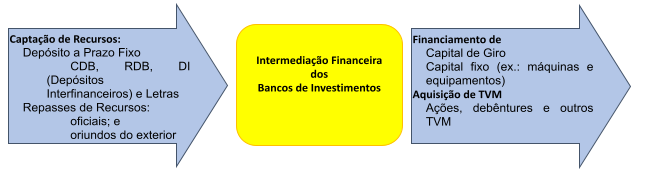
\includegraphics[width=12cm]{banco-investimento}
\centering
\label{banco-invest}
\caption{Fluxo dos Recursos de Intermediação de Bancos de Investimento.}
\end{figure}

Ainda na linha de intermediação financeira, os Bancos de Investimento possibilitam a capitalização de
empresas e a colocação de títulos e valores mobiliários (TVM) para negociação no mercado de capitais.\par

As principais operações são:

\begin{itemize}

  \item o \textbf{underwriting} (subscrição) que é o lançamento (venda) de ações e debêntures de empresas S.A.s para investidores;

  \item a \textbf{securitização de recebíveis} que é a transformação de créditos a receber de empresas
  em títulos negociáveis. Trata-se da liberação do fluxo de caixa de empresas que cedem os direitos
  creditórios (a receber) aos investidores e recebem (na venda) antecipadamente por isso.

\end{itemize}

Os Bancos de investimento são autorizados a prestar serviços relativos aos recursos de terceiros;  entre eles temos:

\begin{itemize}

  \item a \textbf{custódia de valores}, que é o controle (recebimentos de dividendos, de juros, recolhimentos
  de tributos etc.) dos ativos financeiros \textbf{adquiridos diretamente por investidores}, são chamados de serviços de tesouraria e

  \item a \textbf{administração de carteiras de títulos e valores mobiliários}, que é a gestão dos recursos;
  neste caso, o banco de investimento aplica os recursos em ativos financeiros objetivando resultados
  (ganhos). Os fundos de investimentos se enquadram nessa atividade.

\end{itemize}

E, por fim, os \textit{Bancos de Investimentos} são autorizados a realizarem atividades de \textit{Corporate Finance}
que incluem compra e venda de participações, fusões, aquisições e joint ventures.

\section*{Bancos Múltiplos}

Os Bancos Múltiplos são decorrentes da evolução dos conglomerados financeiros no Brasil que, tendo diversas
instituições financeiras sob seu controle, precisavam de maior integração entre as operações e funcionários.\par

A regulamentação, que atendeu as necessidades dos conglomerados financeiros, define que o Banco Múltiplo deve
ser constituído com, no mínimo, 2 carteiras (entre 6 possíveis), sendo uma delas, obrigatoriamente, comercial
e/ou de investimento, e ser organizado sob a forma de sociedade anônima.\par


\begin{table}[H]
\centering
\caption{Instituições Financeiras que podem ser agrupadas para formar um Banco Múltiplo.}
\resizebox{\textwidth}{!}{%
\begin{tabular}{ |p{3cm}|p{3cm}|  }
 \hline
 \textbf{Operações}                                                             & \textbf{Obrigatoriedade}\\
 \hline
 \multicolumn{1}{|l|}{Bancos Comerciais}                                        & \multicolumn{1}{l|}{Sim}\\
 \multicolumn{1}{|l|}{Bancos de Investimentos}                                  & \multicolumn{1}{l|}{}\\
 \multicolumn{1}{|l|}{Sociedades de Crédito Imobiliário}                        & \multicolumn{1}{l|}{Não}\\
 \multicolumn{1}{|l|}{Sociedades de Crédito, Financiamento e Investimento}      & \multicolumn{1}{l|}{}\\
 \multicolumn{1}{|l|}{Banco de Desenvolvimento (apenas para bancos públicos)}   & \multicolumn{1}{l|}{}\\
 \multicolumn{1}{|l|}{Sociedade de Arrendamento Mercantil (Leasing)}            & \multicolumn{1}{l|}{}\\
 \hline
\end{tabular}}
\end{table}


\textbf{Importante}. Quando as Instituições estão agrupadas em forma de Banco Múltiplo, cada operação é chamada
\enquote{carteira}. Cada carteira de um Banco Múltiplo está sujeita às mesmas normas legais e regulamentares
aplicáveis às instituições singulares correspondentes.\par

\section*{Outros Intermediários Financeiros}

\subsection*{Sociedades Corretoras de Títulos e Valores Mobiliários}

As Sociedades Corretoras de Títulos e Valores Mobiliários (CTVM) têm como objetivo intermediar,
nos mercados de bolsa de valores e balcão, operações financeiras com Títulos e Valores Mobiliários (TVM),
metais preciosos e mercadorias (commodities) e moeda estrangeira.\par

Suas principais atribuições são:

\begin{itemize}

  \item operar (acesso aos recintos ou sistemas de negociação) nos Mercados de bolsa, futuros e balcão;

  \item realizar operações de conta margem (depósitos de garantia para operar com os Mercados);

  \item comprar, vender e custodiar TVM, metais preciosos e mercadorias (commodities) por conta própria e por ordem de terceiros;

  \item administrar carteiras (fundos e clubes de investimento);

  \item subscrever (underwriting) emissões e escriturar (manter o controle dos registros) TVM;

  \item exercer funções de agente fiduciário (atua para garantir os direitos dos debenturistas);

  \item emitir certificados de depósito de ações (ações emitidas e negociadas em bolsa estrangeira) e cédulas
  pignoratícias de debêntures (debêntures repassadas em forma de cédula pela instituição);

  \item realizar operações compromissadas (espécie de venda não definitiva, cujo compromisso é recompra do
  ativo em prazo certo e com preço e/ou taxa previamente definidos no início da operação);

  \item intermediar operações de câmbio (a corretora busca, para o cliente, a menor taxa de câmbio
  oferecida pelos Bancos de Câmbio) e

  \item praticar operações no mercado de câmbio de taxas flutuantes (são autorizados a operar, por intermédio
  de um Banco de Câmbio, apenas pequenos negócios equivalentes a US\$$\num{100000}$).

\end{itemize}

Algumas corretoras também prestam serviços de assessoria em investimento com equipes de economistas
próprios ou de empresas terceirizadas.\par

\textbf{Importante}. As CTVMs são autorizadas a funcionar supervisionadas pelo Bacen, contudo suas operações
envolvem TVMs que são disciplinados pela CVM. No que diz respeito à administração de carteiras (fundos e
clubes de investimento) essas atividades são, além de regulamentadas, autorizadas a funcionar exclusivamente pela CVM.\par

As CTVMs \textcolor{red}{\textbf{NÃO PODEM}} fornecer crédito para operações de seus clientes.

\subsection*{Sociedades Distribuidoras de Títulos e Valores Mobiliários}

As Sociedades Distribuidoras de Títulos e Valores Mobiliários (DTVM) têm os mesmos objetivos e, 
praticamente, as mesmas atribuições de uma Corretora (CTVM). As diferenças estão na tabela a seguir:


\begin{table}[H]
\centering
\caption{Diferença entre Corretora e Distribuidora.}
\resizebox{\textwidth}{!}{%
\begin{tabular}{ |p{3cm}|p{3cm}|  }
 \hline
 \textbf{Corretora (CTVM)}                                                             & \textbf{Distribuidora (DTVM)}\\
 \hline
 \multicolumn{1}{|l|}{PODE exercer as funções de agente emissor de certificados 
 e manter serviços de ações escriturais.}                                       & \multicolumn{1}{l|}{Não Pode}\\
 \multicolumn{1}{|l|}{PODE emitir certificados de depósito de ações e cédulas 
 pignoratícias de debêntures.}                                                  & \multicolumn{1}{l|}{Não Pode}\\
 \hline
\end{tabular}}
\end{table}

No passado, a principal distinção entre Corretoras e Distribuidoras era o acesso restrito às 
Corretoras ao recinto de negociação da bolsa (o pregão funcionava na modalidade viva-voz). 
Isso mudou e, atualmente, ambas (Corretoras e Distribuidores) têm acesso para negociação nos 
pregões nos mercados de forma eletrônica.\par

\textcolor{red}{\textbf{Importante}}. Assim como as CTVMs, as DTVMs são autorizadas a funcionar, supervisionadas pelo Bacen, 
contudo suas operações envolvem TVMs que são disciplinados pela CVM. No que diz respeito à administração de carteiras 
(fundos e clubes de investimento), essas atividades são, além de regulamentadas, autorizadas a funcionar exclusivamente pela CVM.\par

\end{document}
